% !TEX root = ../partial-sdm.tex

One particular analysis of Kanerva's interest is given by the limits of recovery.  That is, given an item read at a distance $x$ from a previously stored $\eta$, does this reading at a $\eta_x$ recover the original? Suppose an SDM is trying to read an item written at $\eta$, but the cues received so far lead to a point of distance $x$ from $\eta$.  As one reads at $\eta_x$, a new bitstring $\beta$ is obtained, leading to Kanerva's question: what is the new distance from $\eta$ to $\beta$? Is it smaller or larger than $x$? That, of course, depends on the ratio between $x$ and the number of dimensions of the memory.

\citet[p.70]{Kanerva1988} originally predicted a \textasciitilde 500-bit distance after a point (Figure \ref{fig:kanerva-figure-7.3}). The original prediction considered that the read distance would decline when inside the critical distance and increase afterwards, converging to a \textasciitilde 500-bit distance.  At this point, each read would lead to a different, orthogonal, \textasciitilde 500-bit distance bitstring. He analyzed specifically an SDM with 1,000 bits and 10,000 random bitstrings written into it.

\begin{figure}[h]
\centering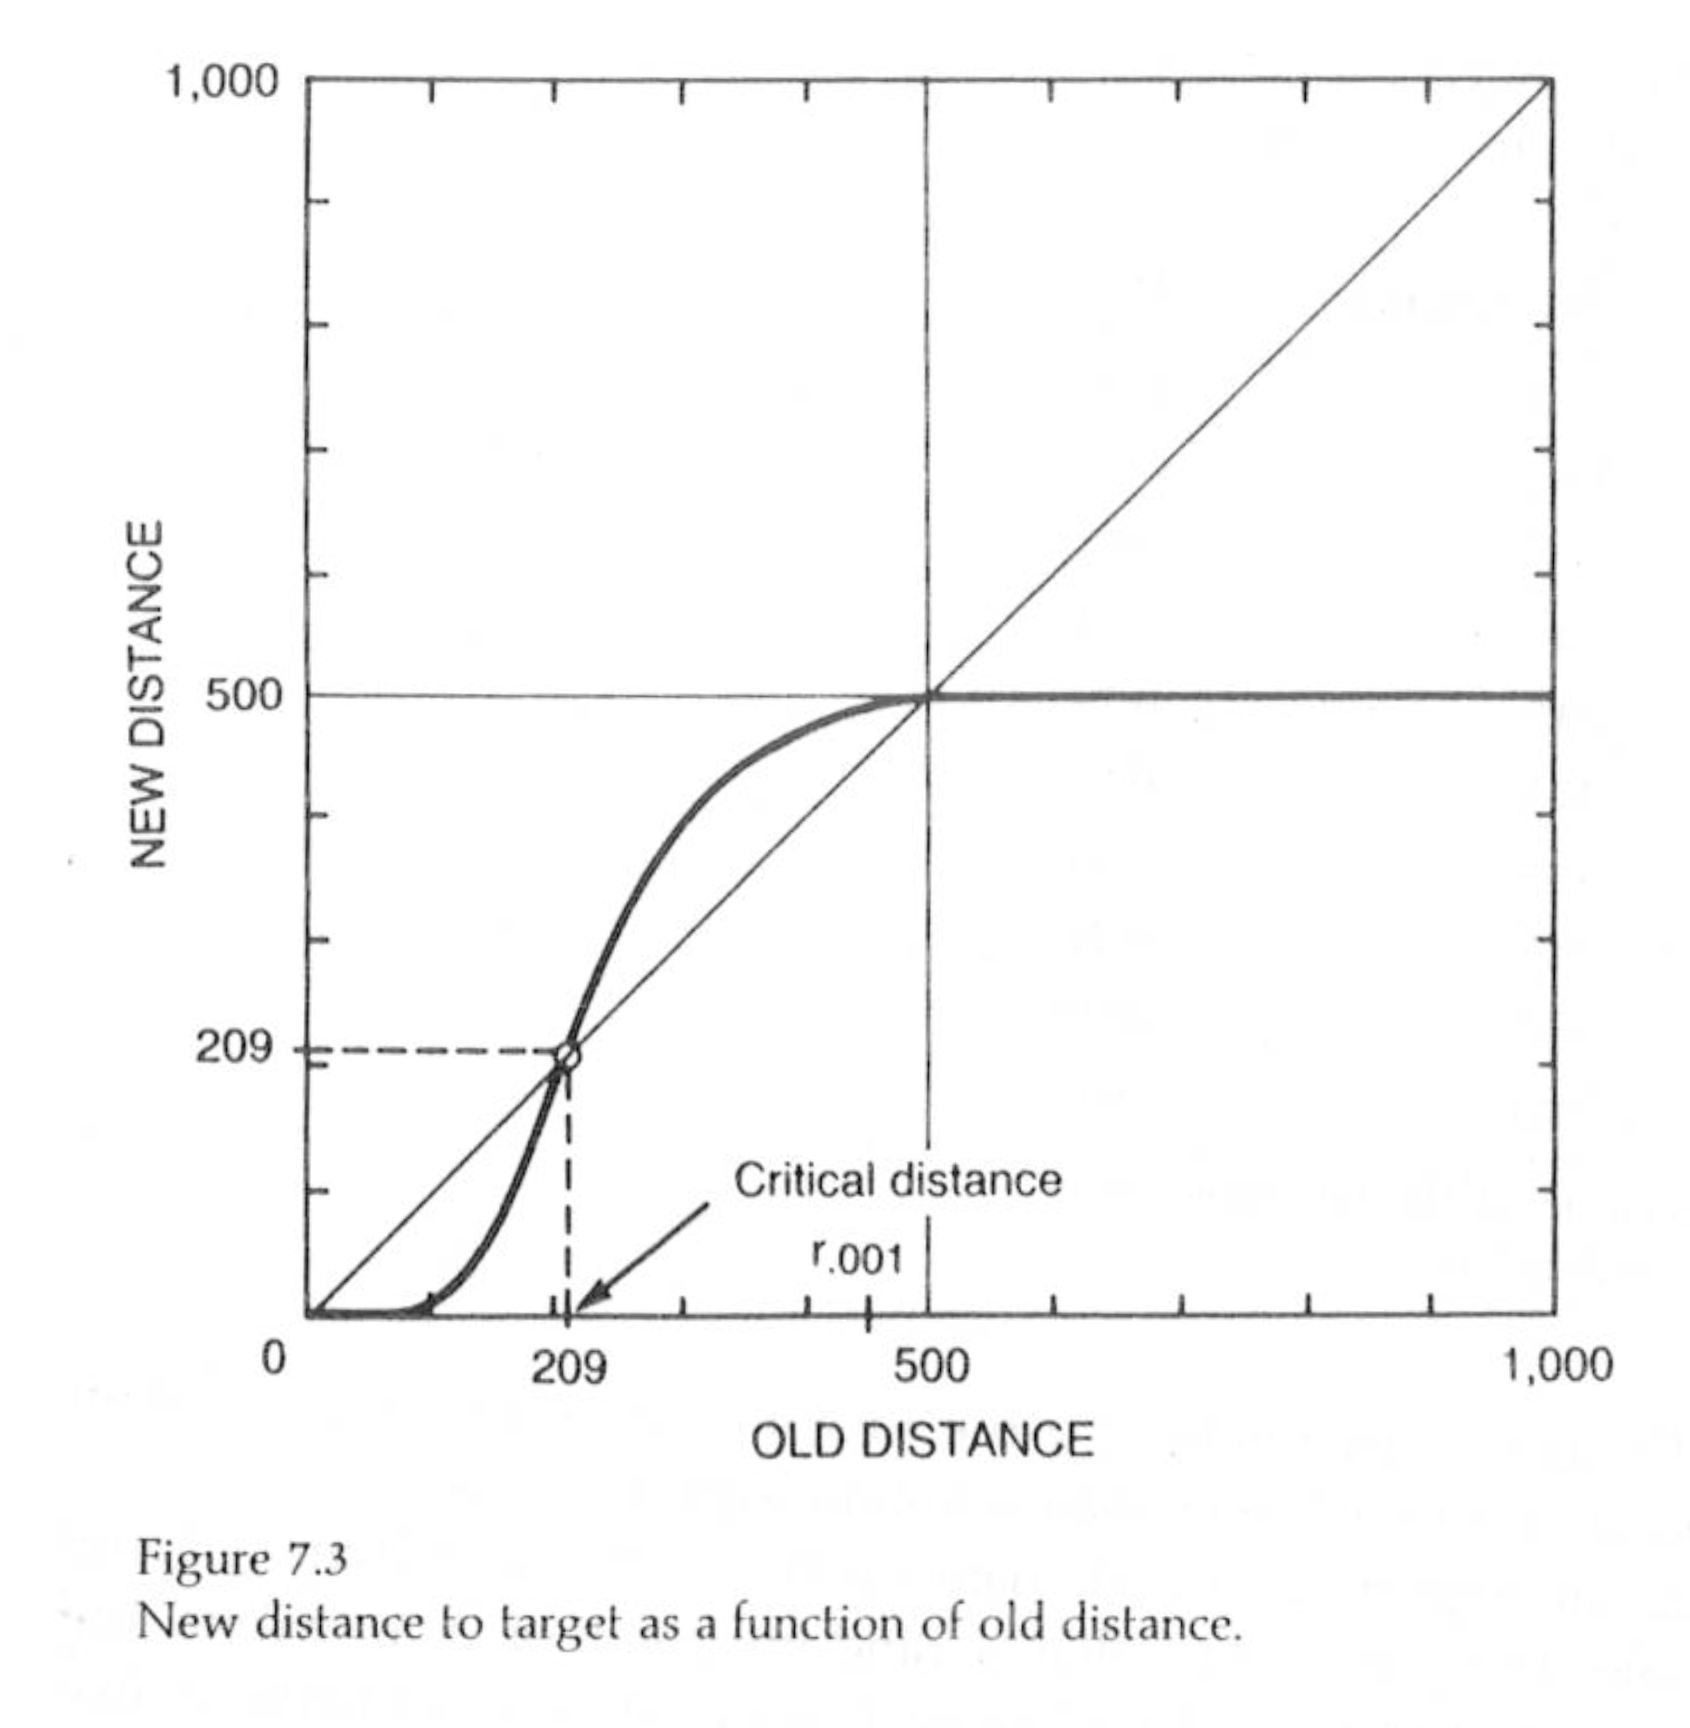
\includegraphics[width=0.8\textwidth]{images02/kanerva-table-7-2-original.png}
\caption{Kanerva's original Figure 7.3 (p. 70) predicting a \textasciitilde 500-bit distance after a point.
\label{fig:kanerva-figure-7.3}}
\end{figure}

As we ran the simulations, this one in particular struck our attention: The new distances obtained after a read operation were not perfectly predicted by the theoretical model. We have strictly followed Kanerva's configuration and, even so, we have found out some deviations from Kanerva's original theoretical analysis and the results obtained by simulation.

In details, we have created a SDM with $n=1,000$, $H=1,000,000$, and $r=451$. Then, we have generated 10,000 random bitstrings and written them into the memory. Then, we have generated a reference bitstring (bs\_ref) and written it into the memory. Then, we have executed the following steps with $x$ from 0 to 1,000: (i) copy bs\_ref into a new bitstring; (ii) randomly flipped $x$ bits of the copy; (iii) read from the memory in the copy address; and (iv) stored the distance between the returned bitstring and bs\_ref. Finally, we have plotted Figure \ref{fig:sdm-10000w-table-7-2}.

\begin{figure}[h]
\centering
\subfloat[1 sample for each distance $x$ \label{fig:sdm-10000w-table-7-2-1sample} ]{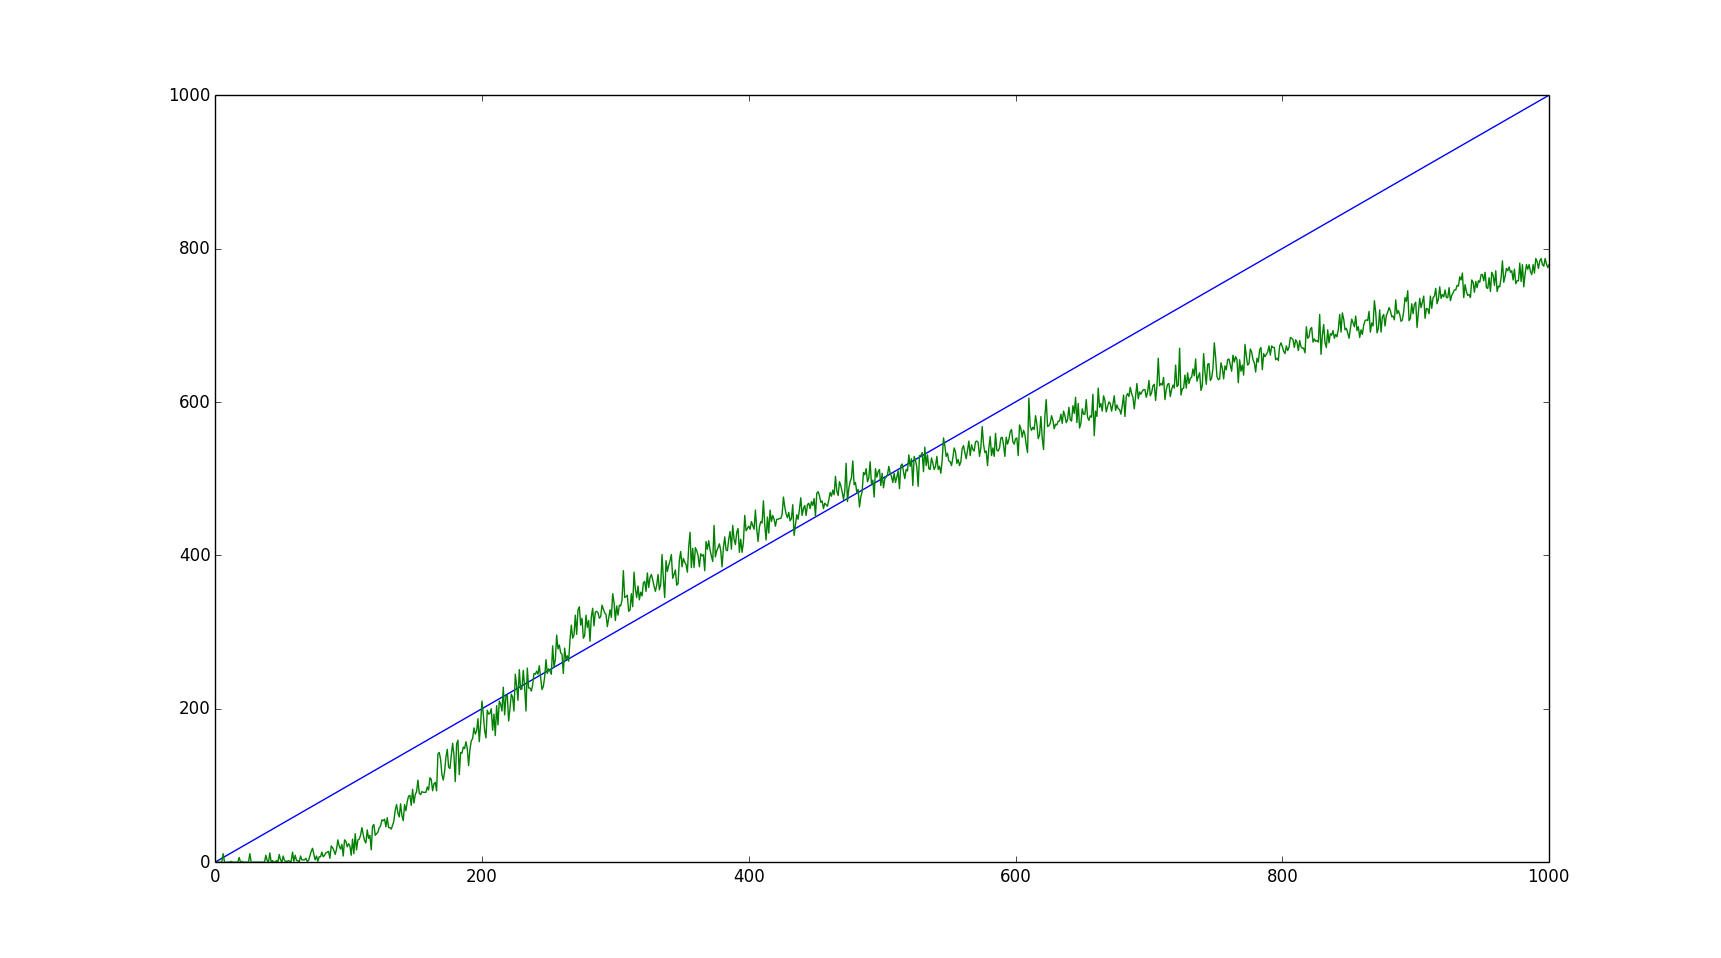
\includegraphics[width=0.5\textwidth]{./images02/sdm-10000w-table-7-2.png}}
\subfloat[6 samples for each distance $x$ \label{fig:sdm-10000w-table-7-2-6samples} ]{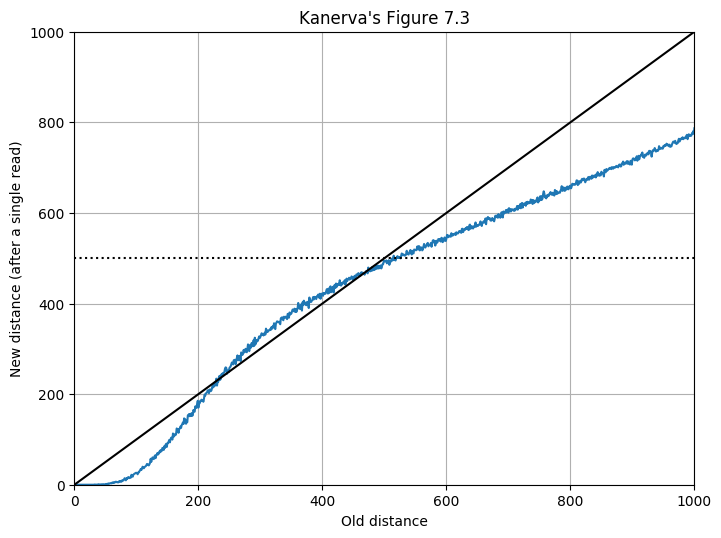
\includegraphics[width=0.5\textwidth]{./images02/sdm-10000w-table-7-2-6-samples.png}}

\caption{Results generated by the framework diverging from Kanerva's original Table 7.2. Here we had a 1,000 bit, 1,000,000 hard-location SDM with exactly 10,000 random bitstrings written into it, which was also Kanerva's configuration.
\label{fig:sdm-10000w-table-7-2}}
\end{figure}

Figure \ref{fig:sdm-10000w-table-7-2-1sample} has a lot of noise because we have read only once for each distance $x$ and Kanerva has predicted the average distance. So, we have changed the steps to run $k$ reads and store the average new distance. We run with $k=6$, and the results can be seen in Figure \ref{fig:sdm-10000w-table-7-2-6samples}, which has much lower noise and still holds the divergence.

Our results show that the theoretical prediction is not accurate.  There are interaction effects from one or more of the attractors created by the 10,000 writes, and these attractors seem to raise the distance beyond \textasciitilde 500 bits (Figure \ref{fig:sdm-10000w-table-7-2}).

Obviously, these small deviations from Kanerva's original theoretical predictions deserve a qualification.  Kanerva was working in the 1980s and the 1990s, and had no access to the immense computational power that we do today. It is no surprise that some small interaction effects should exist as machines allow us to explore the ideas of his monumental work.

But, when we reduced the number of random bitstrings written in the SDM from 10,000 to only 100, the results reflected very well the Kanerva's theoretical expectation (Figure \ref{fig:sdm-100w-table-7-2-10samples}). This result strengthens our hypothesis that the disparities in the computational results are due to the interaction effect of high numbers of different attractors. In Figure \ref{fig:sdm-table-7-2-steps} we can notice that, the more random bitstrings are written, the stronger the attractors.

\begin{figure}[h]
\centering
\subfloat[100 writes \label{fig:sdm-100w-table-7-2-10samples} ]{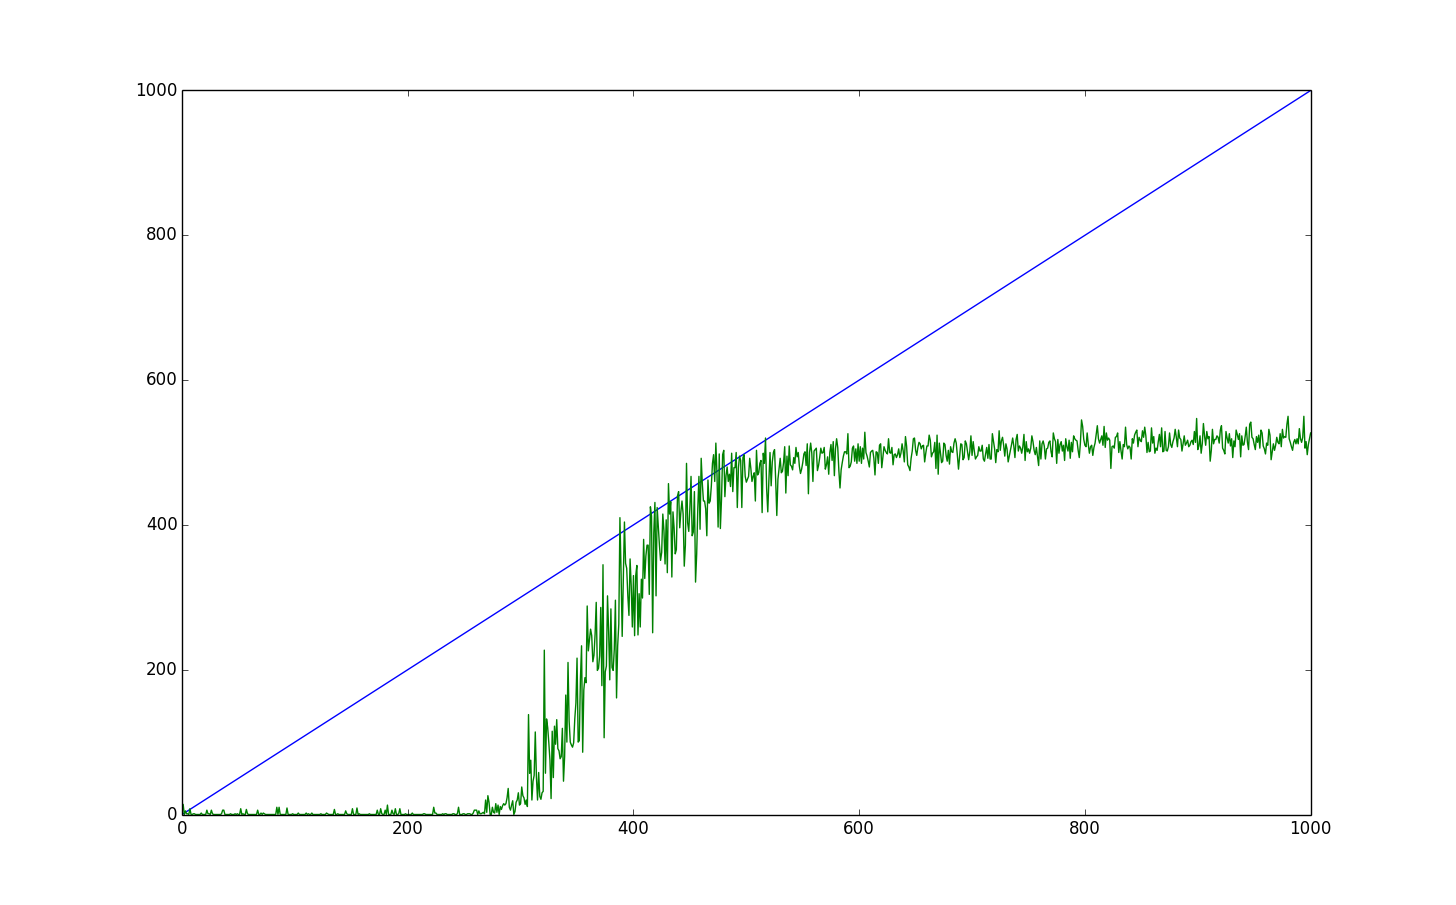
\includegraphics[width=0.47\textwidth]{./images02/sdm-100w-table-7-2.png}}
\subfloat[Steps of 1,000 writes \label{fig:sdm-table-7-2-steps} ]{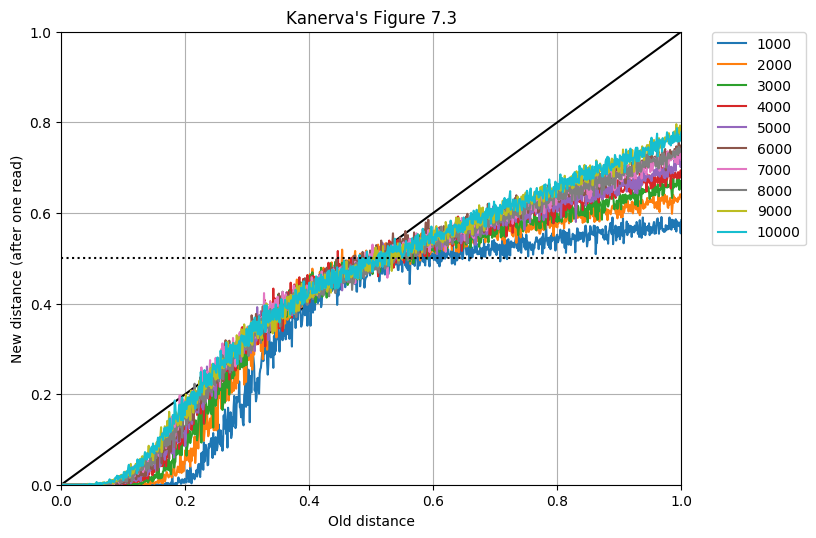
\includegraphics[width=0.53\textwidth]{./images02/sdm-table-7-2-steps.png}}
%\centering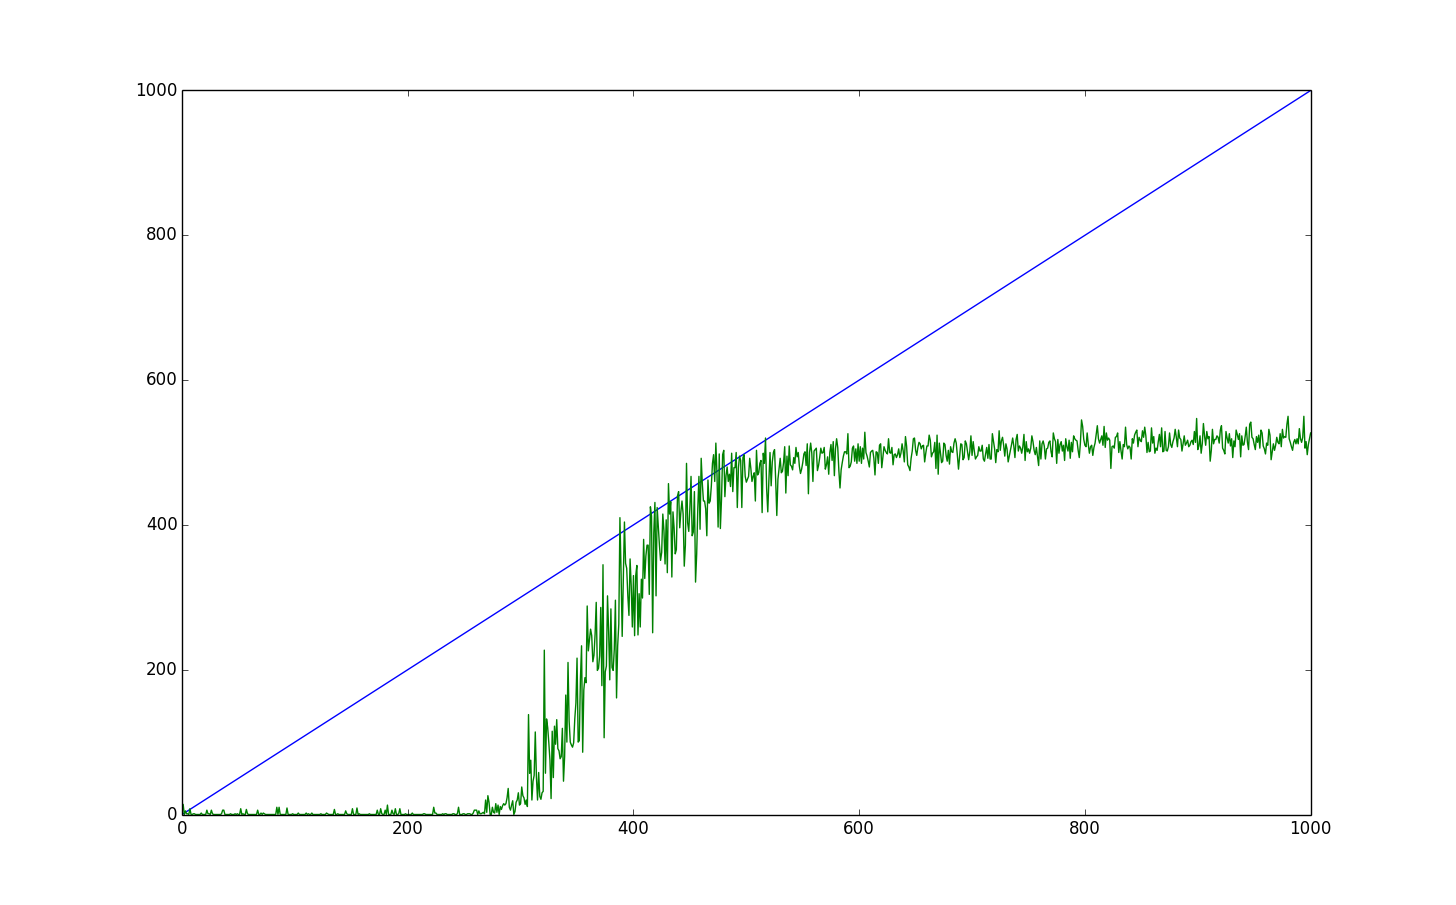
\includegraphics[width=\textwidth]{images02/sdm-100w-table-7-2.png}

\caption{Results generated by the framework similar from Kanerva's original Table 7.2. Here we have a 1,000 bit, 1,000,000 hard-location SDM with (a) exactly 100 random bitstrings written into it and (b) steps of 1,000 random bitstrings written into it.
\label{fig:sdm-100w-table-7-2}}
\end{figure}

To obtain the results from Figures \ref{fig:sdm-10000w-table-7-2} and \ref{fig:sdm-100w-table-7-2}, we had to write 10,000 random bitstrings to an SDM, and then randomly choose one of those bitstrings to be our origin. Finally, we randomly flipped some bits from the origin bitstring and executed a reading operation in the SDM. Thereby, in order to show the interaction effects more clearly, we changed the single read for an 15-iterative read. As we can see in Figure \ref{fig:sdm-10000w-table-7-2-15iter}, after a distance of 500 bits, all bitstrings converged to 500-bit distance bitstrings, just as described by Kanerva.

Hence, our understanding is that the attractors are just preventing the bitstrings to converge directly to 500-bit distance bitstrings, requiring more reading steps to do so. They are in other orthogonal bitstrings' critical distance, but sufficiently far not to converge in a single read.

\begin{figure}[h]
\centering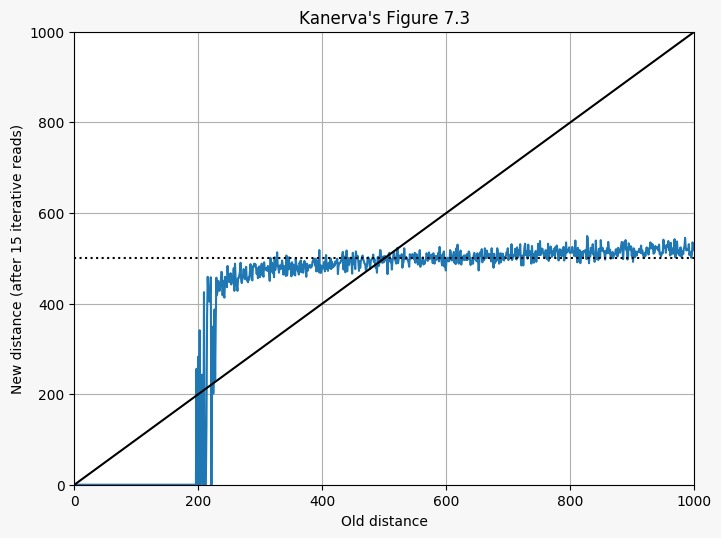
\includegraphics[width=\textwidth]{images02/sdm-10000w-table-7-2-15iter.png}
\caption{This graph shows the interaction effects more clearly.  As we change the single read to a 6-iterative read, the effect has vanished and all bitstrings above $x=500$ have converged to 500-bit distance bitstrings. Here we have the exact same configuration of Figure \ref{fig:sdm-10000w-table-7-2}, except for the iterative read.
\label{fig:sdm-10000w-table-7-2-15iter}}
\end{figure}

Going further in the analysis, we calculated the probability of missing a bit when reading from SDM. After all, that's how Kanerva has originally found the curve. To do this, we used the following equations from our previous work \citep{brogliato2014sparse}. Let $d$ be the distance to the target, $h$ be the number of hard-locations activated during read and write operations, $s$ be the number of total stored bitstrings, $H$ be the number of total hard-locations, $w$ be the number of times the target was written into SDM, $\theta$ be the total random bitstrings in all $h$ hard-locations activated by read operation, and $\phi(d)$ be the average number of shared hard-locations activated two bitstrings $d$ bits away.

\begin{align}
\theta &= \frac{sh^2}{H} - w \cdot \phi(d) \\
P(miss | bit=0) &= 1 - P \left( \sum_{i=1}^\theta X_i < \frac{sh^2}{2H} \right) \\
P(miss | bit=1) &= P \left( \sum_{i=1}^\theta X_i < \frac{sh^2}{2H} - w \cdot \phi(d) \right) \\
P(miss) &= \frac{1}{2} \cdot \left[ P(miss | bit=0) + P(miss | bit=1) \right]
\end{align}

For details and the proof of this equation, see \citet{brogliato2014sparse}. Although Kanerva has found a formula for $\phi(d)$ through an unsolved integral, and \citet{de1995geometrical} have proposed another way to calculate $\phi(d)$, we have used our framework to estimate the values of $d$. In order to do that, we used a Monte Carlo approach, generating many pair of random bitstrings $d$ bits away from them and calculating the average number of shared hard-locations between them. The code is available in the ``Calculate critical distance'' notebook \citep{sdmframework}.

Kanerva's settings according to the parameters of the equation were: $s=10,000$, $H=1,000,000$, and $w=1$. We have calculated $\phi(d)$ as explained, and $h = H \cdot 2^{-n} \sum_{i=0}^{r} \binom{n}{i}$, where $n=1,000$ and $r=451$. Finally, $h=1,071.85$ and changing $d$ from $0$ to $1000$, we got Figure \ref{fig:kanerva-figure-73-calculated}.

\begin{figure}[!htb]
\centering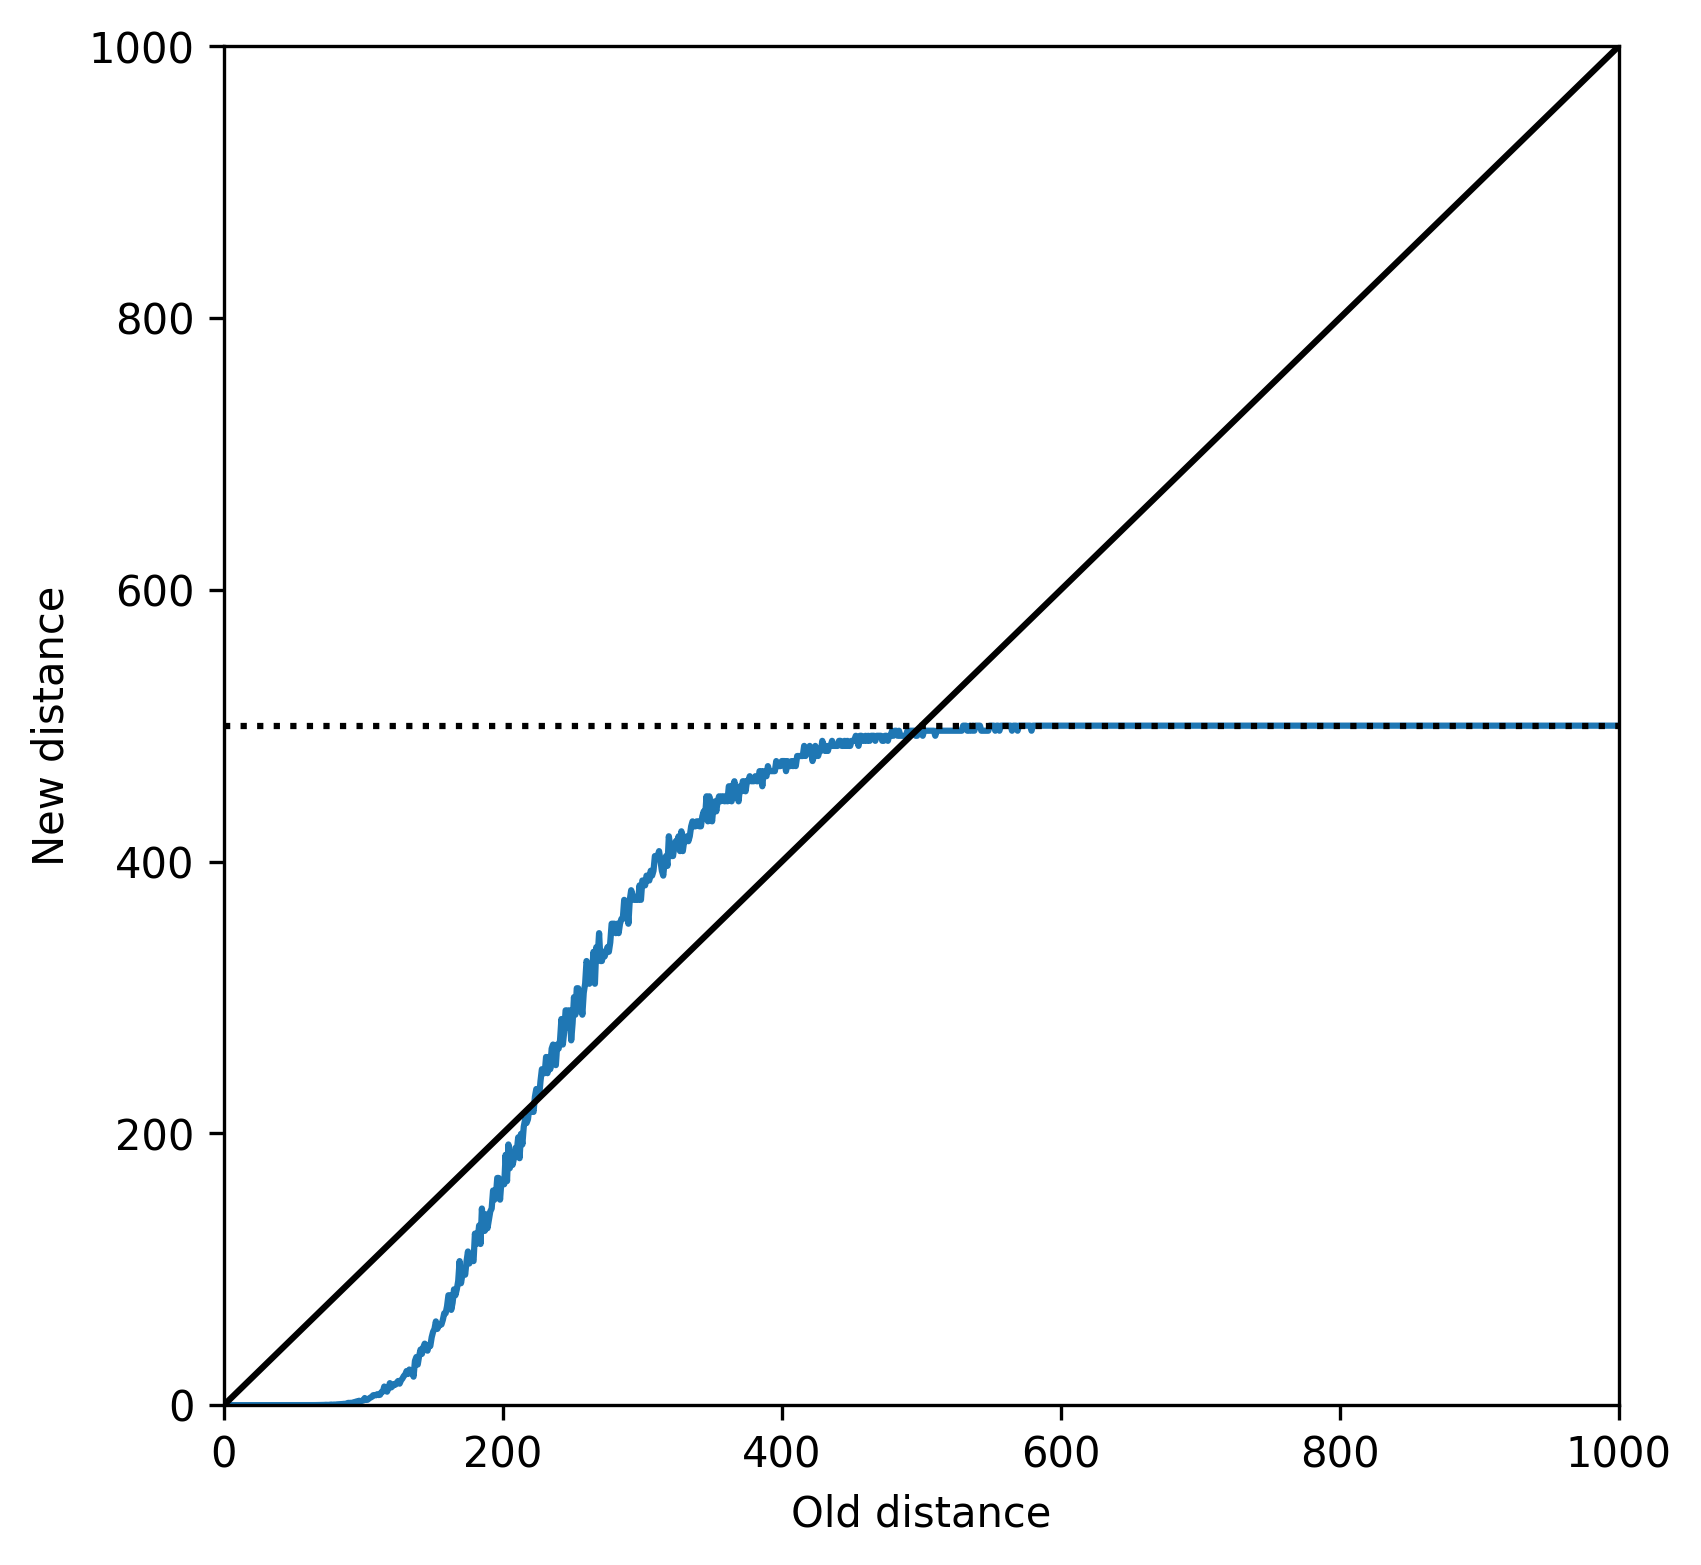
\includegraphics[width=0.8\textwidth]{./images02/calculated-table-72.png}
\caption{Kanerva's original Figure 7.3 generated using the equations from \citet{brogliato2014sparse}.
\label{fig:kanerva-figure-73-calculated}
}
\end{figure}

As we can easily notice, we got exactly the same curve as Kanerva. This question has been intriguing us since then and we are still looking for a more analytic explanation then merely interference from the other written attractors.


\section{Critical distance of 209}

The critical distance is defined as $d$ where $P(miss) = d/n$, or, in Figure \ref{fig:kanerva-figure-73-calculated}, the point where the curve meets with the identity function (the black diagonal line). Thus, we plot a zoom-in of Figure \ref{fig:kanerva-figure-73-calculated} around $d=209$ in Figure \ref{fig:figure-73-eq-zoom-in} using the same equations \citep{brogliato2014sparse}. It was surprising that the meeting does not happen at $d=209$, but around $d=221$.

\begin{figure}[!htb]
\centering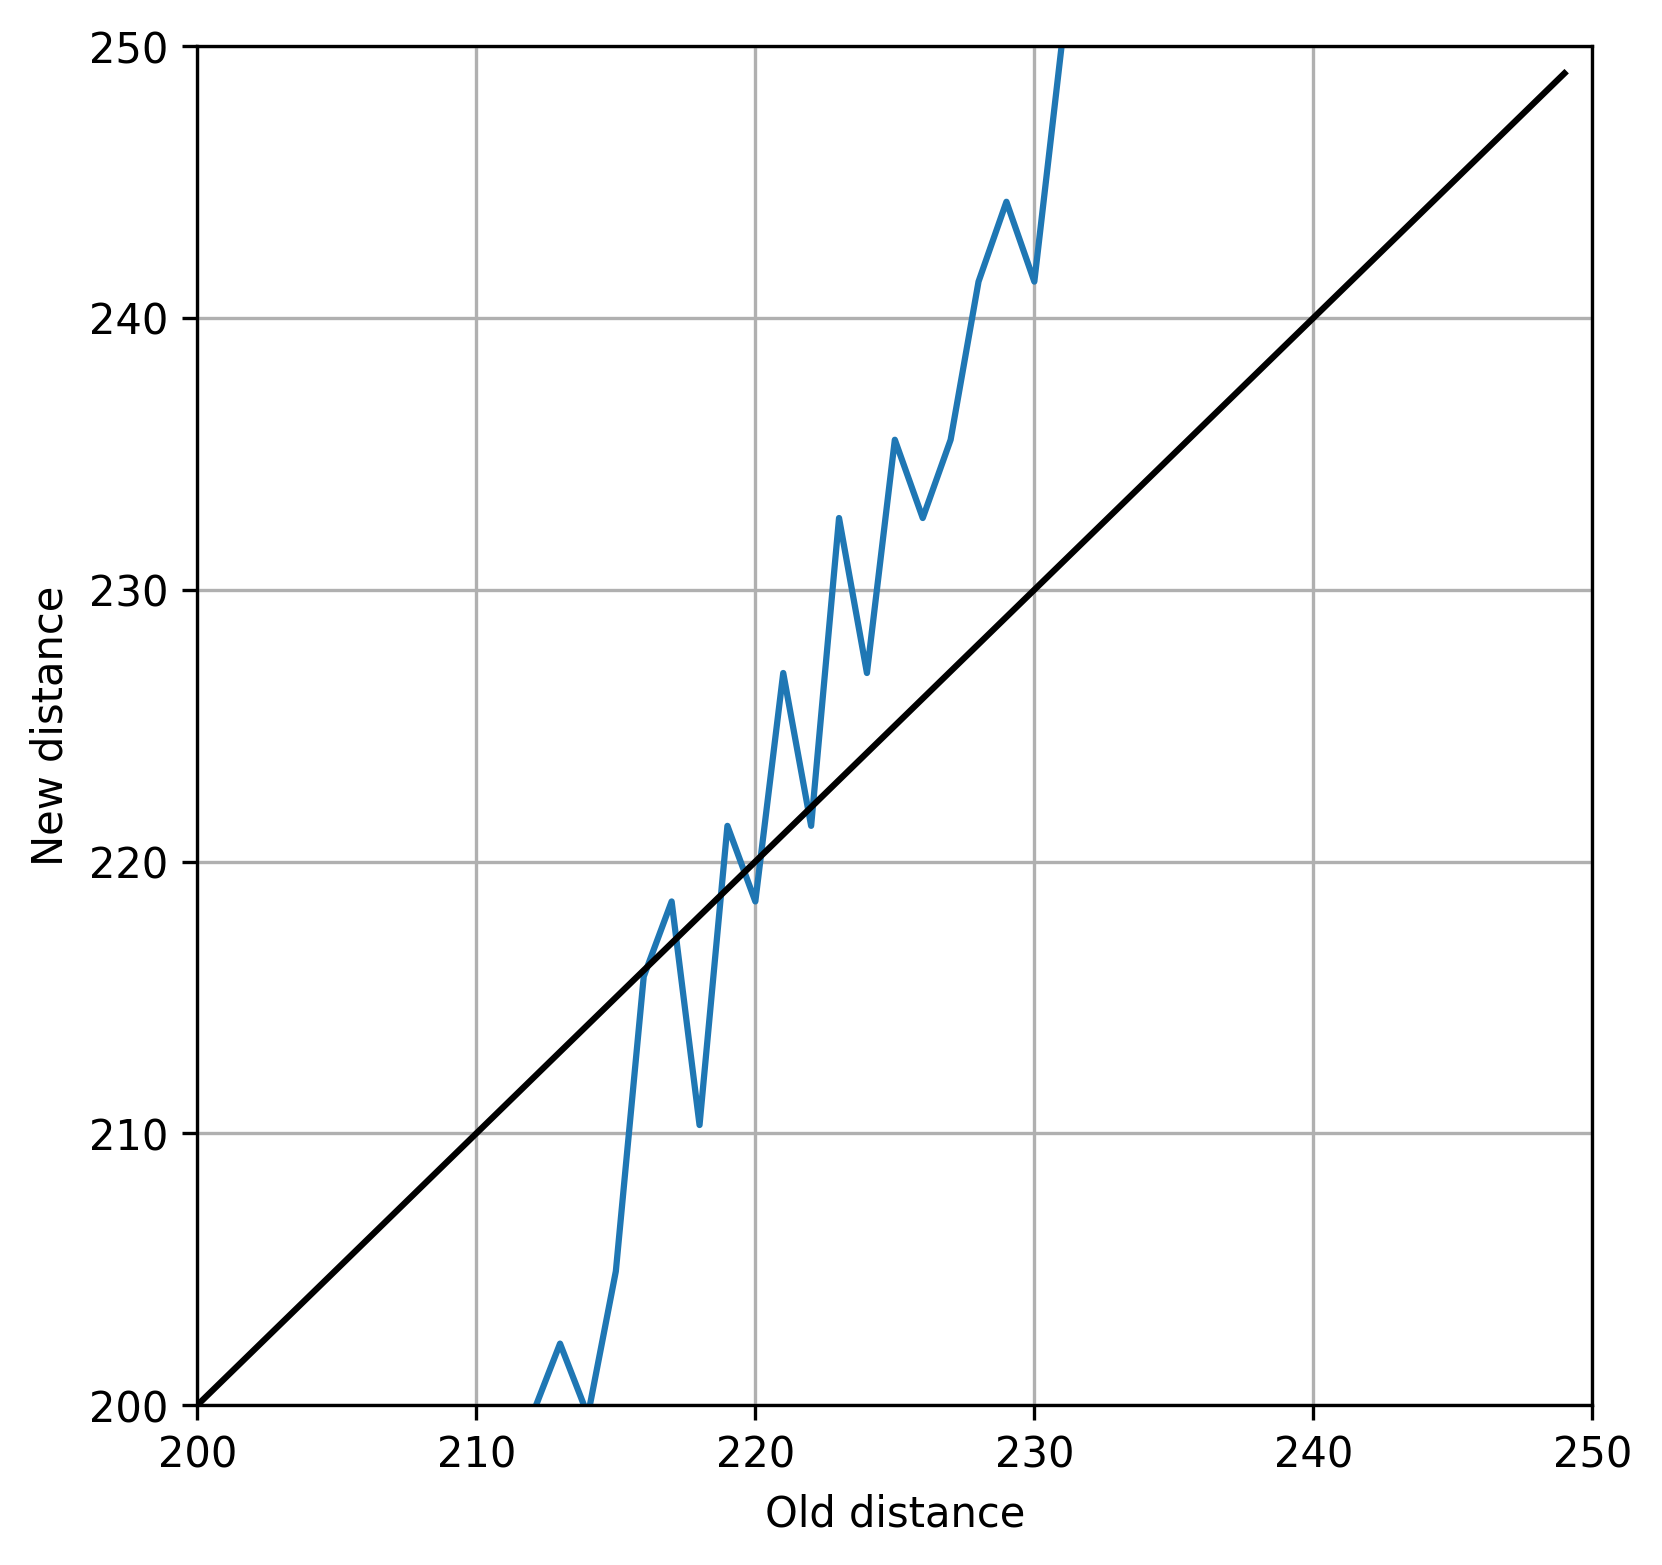
\includegraphics[width=0.8\textwidth]{./images02/figure-73-eq-zoom.png}
\caption{Zoom-in around $d=209$ of Figure \ref{fig:kanerva-figure-73-calculated}.
\label{fig:figure-73-eq-zoom-in}
}
\end{figure}

To confirm that the critical distance is not around 209, but around 221, we also plot a zoom-in of Figure \ref{fig:sdm-10000w-table-7-2} around $d=209$ in Figure \ref{fig:sdm-10000w-zoom}. In order to reduce the noise, we increased the samples to $k=180$.

\begin{figure}[!htb]
\centering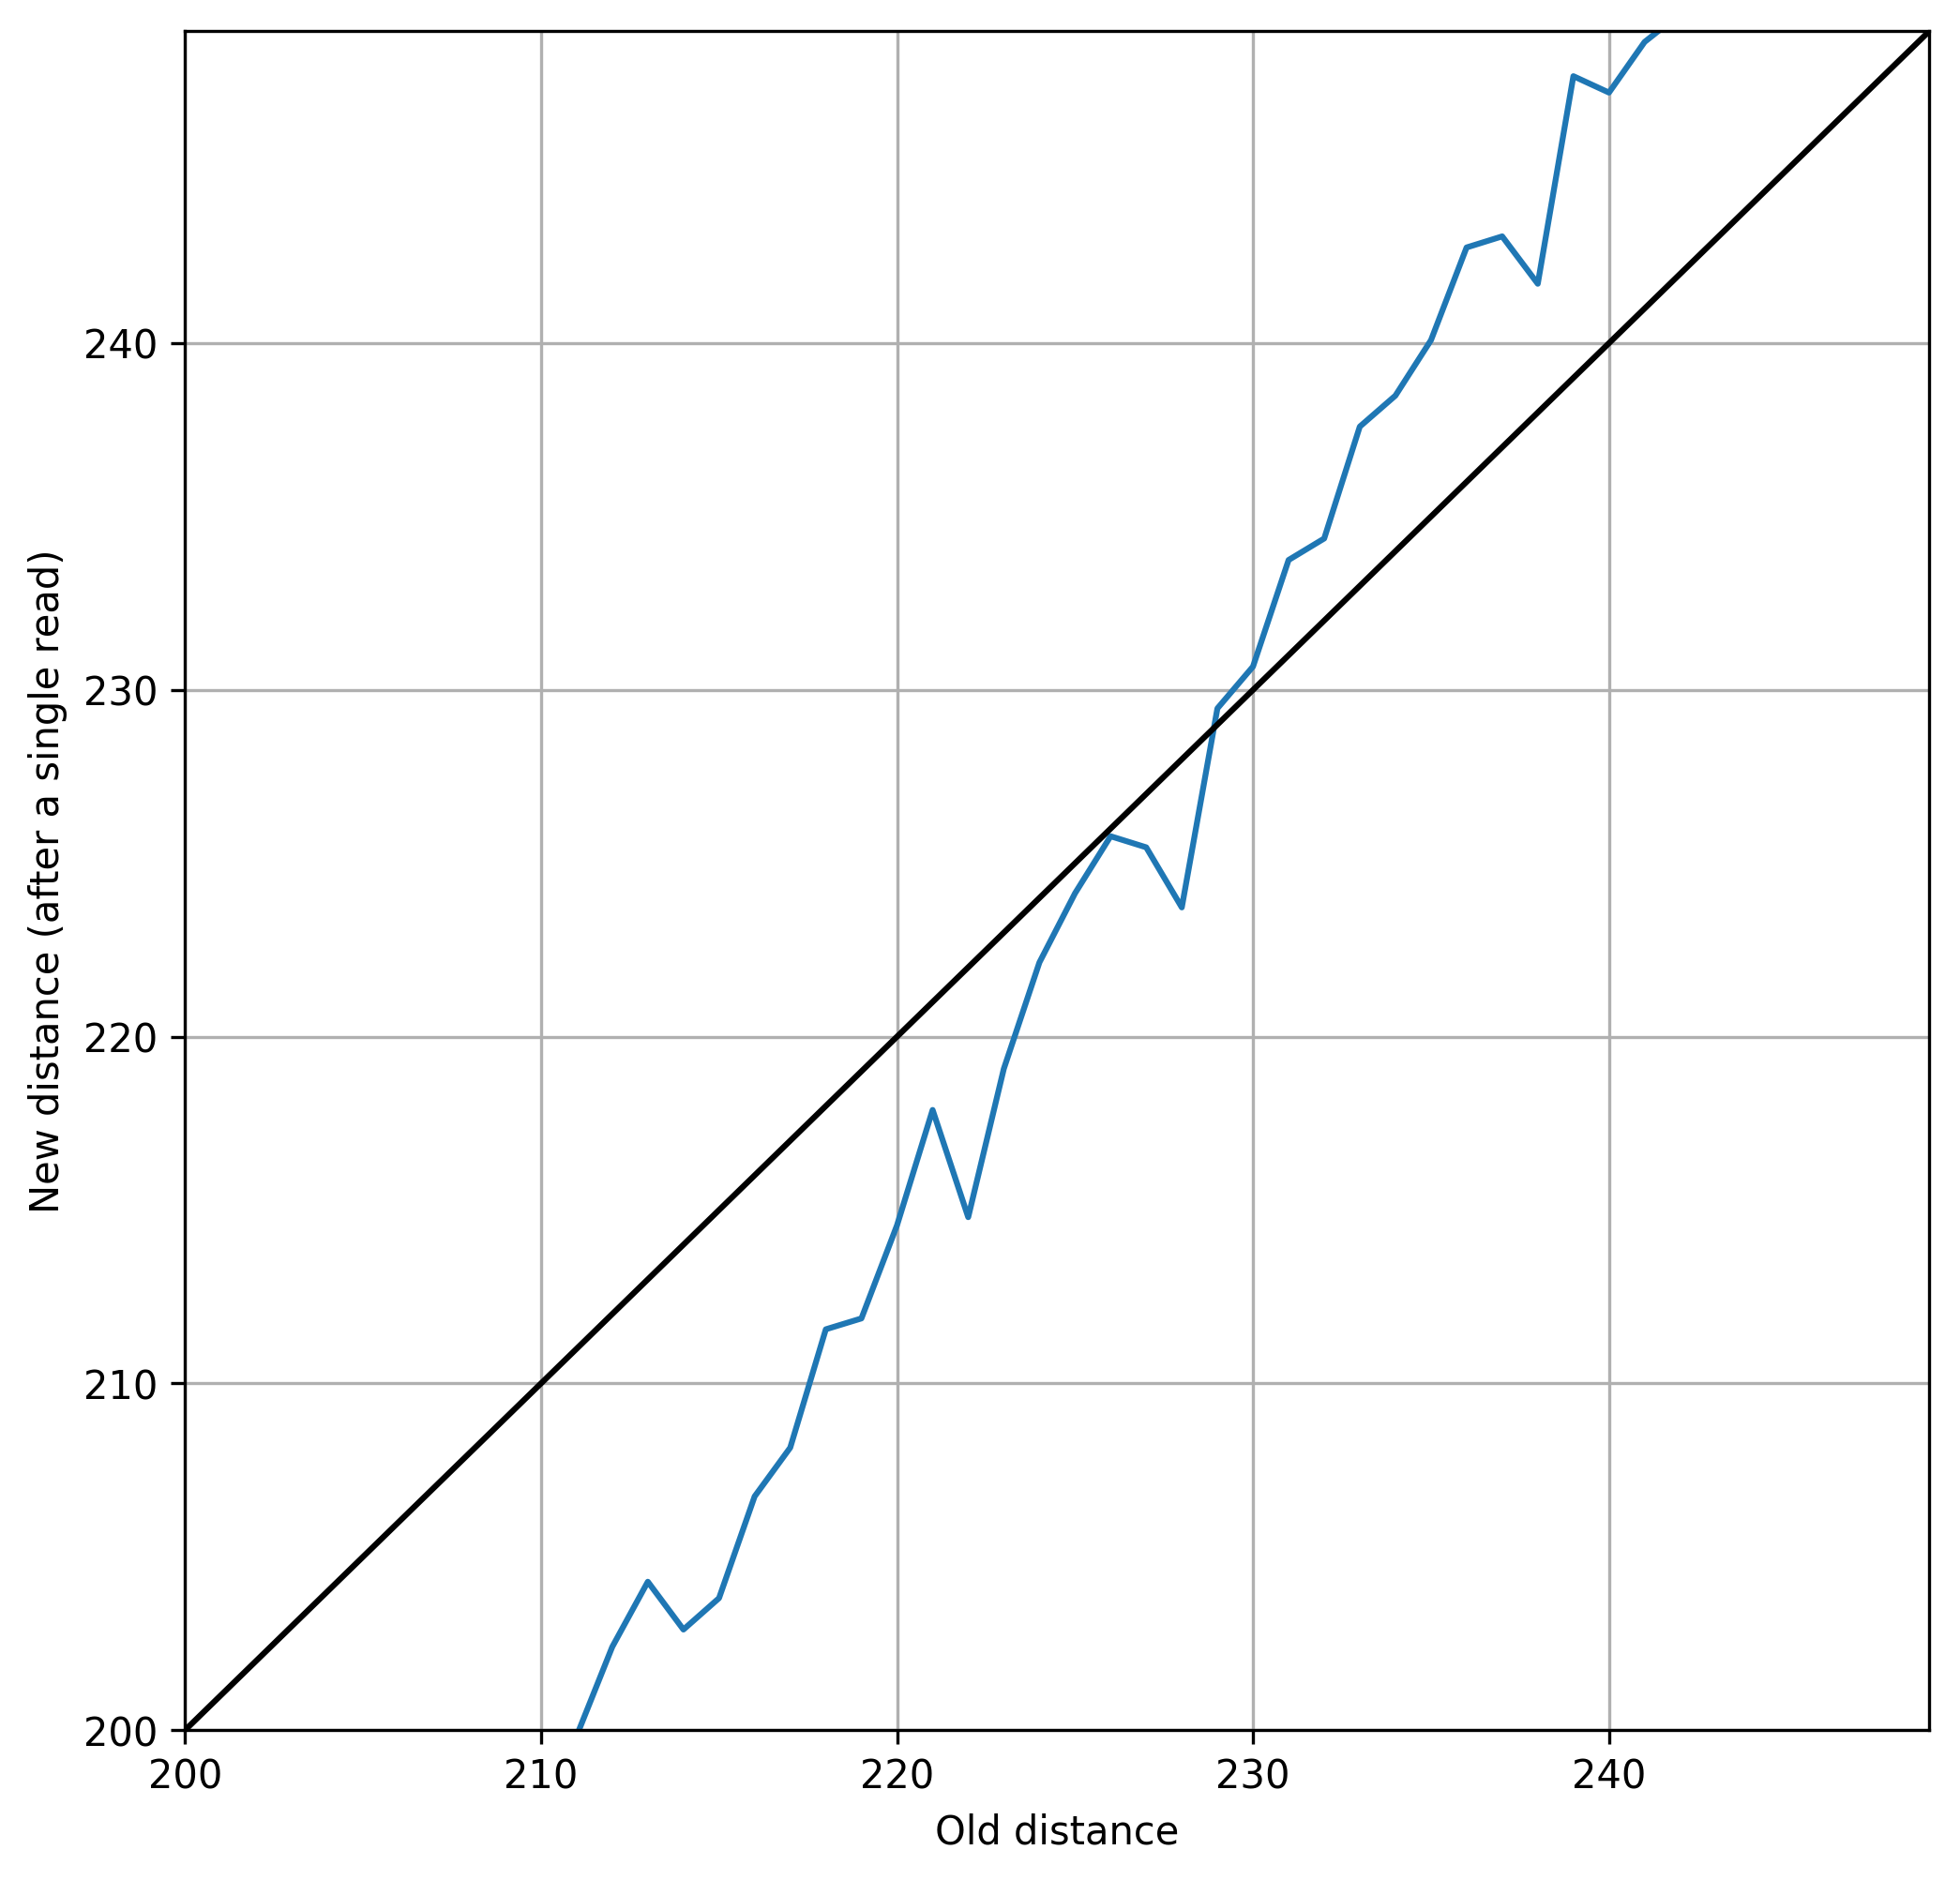
\includegraphics[width=0.8\textwidth]{./images02/sdm-10000w-zoom-209.png}
\caption{Zoom-in around $d=209$ of Figure \ref{fig:sdm-10000w-table-7-2}.
\label{fig:sdm-10000w-zoom}
}
\end{figure}


%To obtain the results from Figures \ref{fig:sdm-10000w-table-7-2} and \ref{fig:sdm-100w-table-7-2}, we had to write 10,000 random bitstrings to an SDM, and then randomly choose one of those bitstrings to be our origin. Finally, we randomly flipped some bits from the origin bitstring and executed a reading operation in the SDM. Thereby, in order to show the interaction effects more clearly, we wrote a handmade bitstring to the SDM which had all bits inverted in relation to the origin bitstring --- their hamming distance was equal to 1,000. Our handmade bitstring was acting as an opposite attractor, and one can see the accelerating effects towards convergence to both attractors: the origin and the handmade bitstrings (Fig. \ref{sdm-10000w-notX-table-7-2}). Here we had the exact same configuration of Figure \ref{sdm-10000w-table-7-2}, with the addition of the single opposite attractor.

%\begin{figure}[h]
%\centering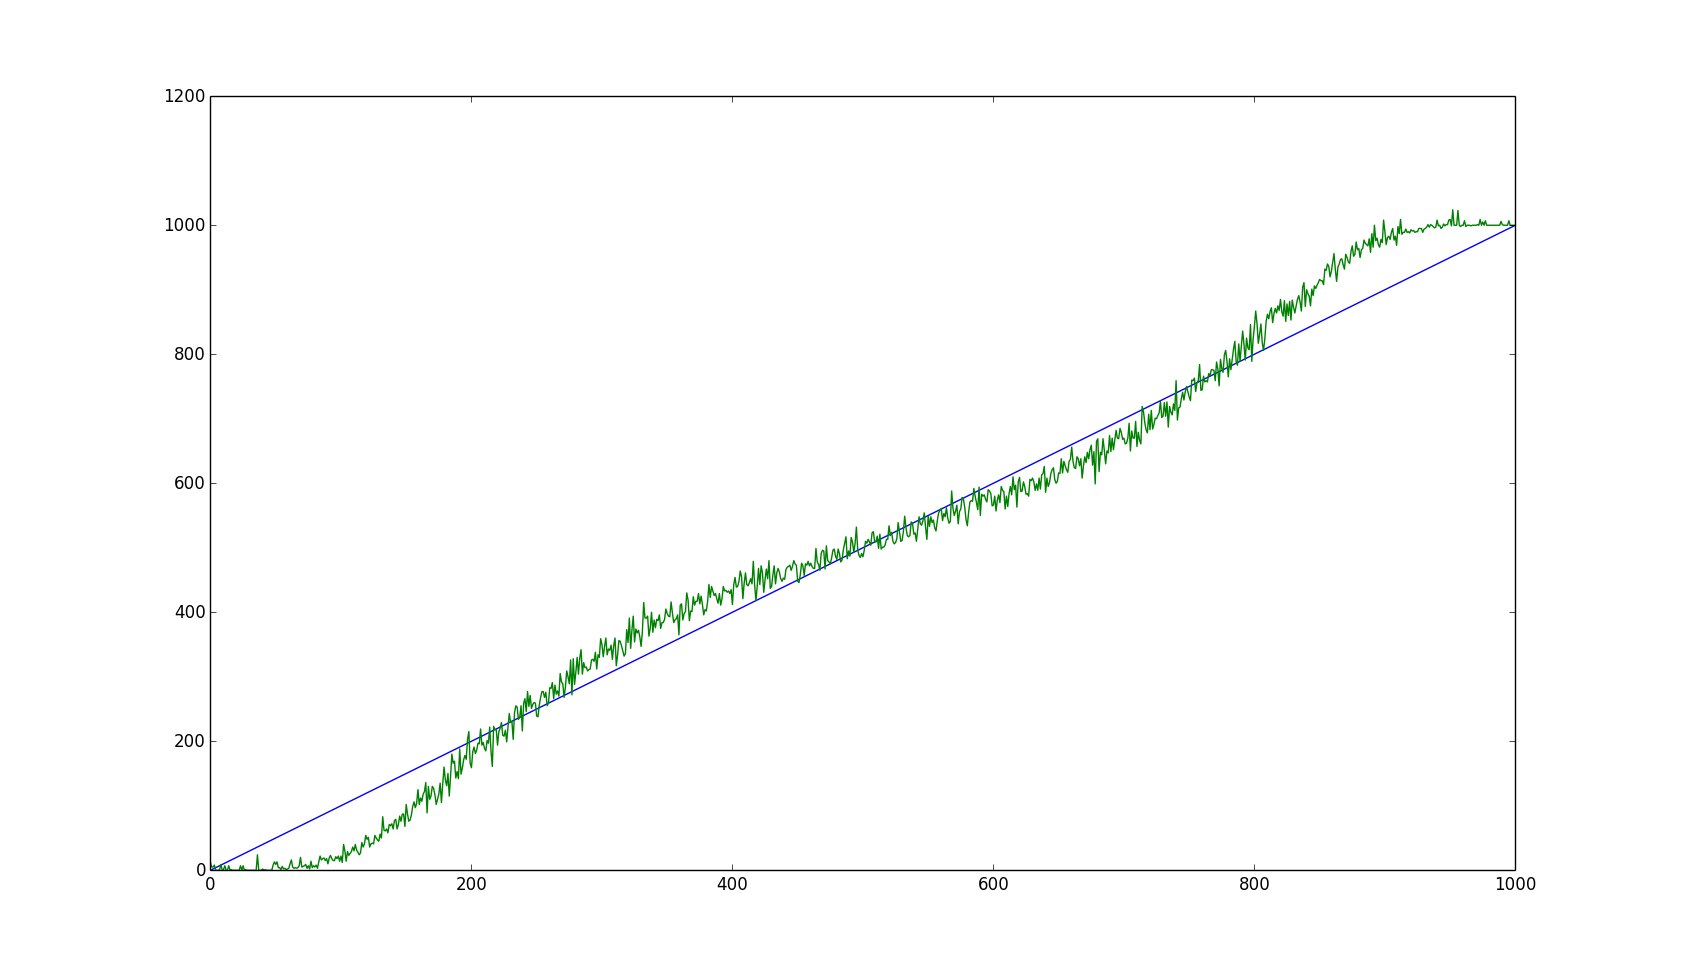
\includegraphics[width=0.8\textwidth]{images02/sdm-10000w-notX-table-7-2.png}
%\caption{This graph shows the interaction effects more clearly.  As we include an opposite bitstring, one can see the accelerating effects towards convergence to both attractors: the origin and its polar opposite. Here we have the exact same configuration of Figure \ref{sdm-10000w-table-7-2}, with the addition of the single opposite attractor.
%\label{sdm-10000w-notX-table-7-2}}
%\end{figure}
